% !TEX root = ../main.tex
\chapter{Detailed design}

This chapter details further the architecture described in the previous one, explaining the choices that shaped each
part of the obtained design, the patterns those choices led to. The descriptions are divided by the layer they belong to.
Diagrams are included to explain in more detail the relationship.

The key choice that led to this architecture and the following design is that everything in the model is a value, and
every operation upon one yields another value, rather than altering what it was given.

\section{Model}

The model holds every rule of the game and nothing else. It opens no file, draws nothing, and uses no library beyond
Scala's own and a few types from the Java platform.

Two decisions shaped it. The first is that a level, that is the whole state of a game at one instant, is a single value
from which the next is computed. For this reason, everything in the model must compose into that value, and nothing in
it can keep a state of its own. The second is the requirement that the behavior of modes and enemies must be extensible.
This led to each of them being expressed as something to be implemented: a new mode or a new enemy behavior is written
on its own, leaving the rules already written untouched.

\subsection{Value objects and semantics}

Everything in the model is a value, something entirely defined by its contents, using which it can be compared to other
values, rather than relying on IDs, and it is immutable. Immutability was employed as much as possible, not limiting it
to positions and movements but to whole game states being considered as single values, so that no part of the model can
have a state of its own.

Values carry the small operations that belong to them, rather than leaving those to their callers. A direction added to
a position returns an adjacent position. A movement advanced by a duration gives the movement further along, or reports
that it has arrived. The arithmetic of the maze lives with the values it concerns, and the rules above are written in
terms of positions and movements rather than rows and columns.

What follows is that a whole game can be compared with ordinary equality, allowing, for example, saved games to be
tested by asserting that what was read back equals what was written, with no need for the comparison to be written by
hand.

The cost is that every update allocates rather than overwrites, creating a stream of short-lived values. This is
accepted, as the cost of a complete update is reported in the chapter on testing, and is well within the time a
frame allows.

\subsection{Constructing valid values}

\subsection{Level State}

\subsection{Effects}

\subsection{Entities and their movement}

Both the player and the enemy can be similarly described as entities that occupy a cell in the maze, face a certain
direction, and may be moving, meaning that they might be in-between adjacent cells. The cell they occupy is discrete,
and changes only upon arrival of the entity on a different cell. The crossing from a cell to an adjacent one is held
separately, as the movement that is being performed and the time left to complete it. This lets the position always be
whole. Only the drawing interpolates, and based on the crossing behavior rather than from the position of the entities.

Speed is expressed as the time taken to cross one cell, rather than as a distance to be covered per update, making an
entity faster than another on the basis of a model choice rather than frame rate.

An entity is not aware of the maze. When asked to move, it is handed a predicate that determines which positions are
walkable, and refuses the step if the answer is negative. The same type therefore serves the player and the enemies,
without either knowing what it is moving through, and can be exercised in tests against predicates written by hand.

The event of two entities meeting is not simply them sharing a cell, but also two entities swapping their respective
positions at the same time. Therefore, an entity remembers the cell it most recently left, and thus a meeting is
recognized in three ways: two entities occupy the same cell, two entities crossing into each other's cells, or two
entities standing where each other just was.

\begin{figure}
    \centering
    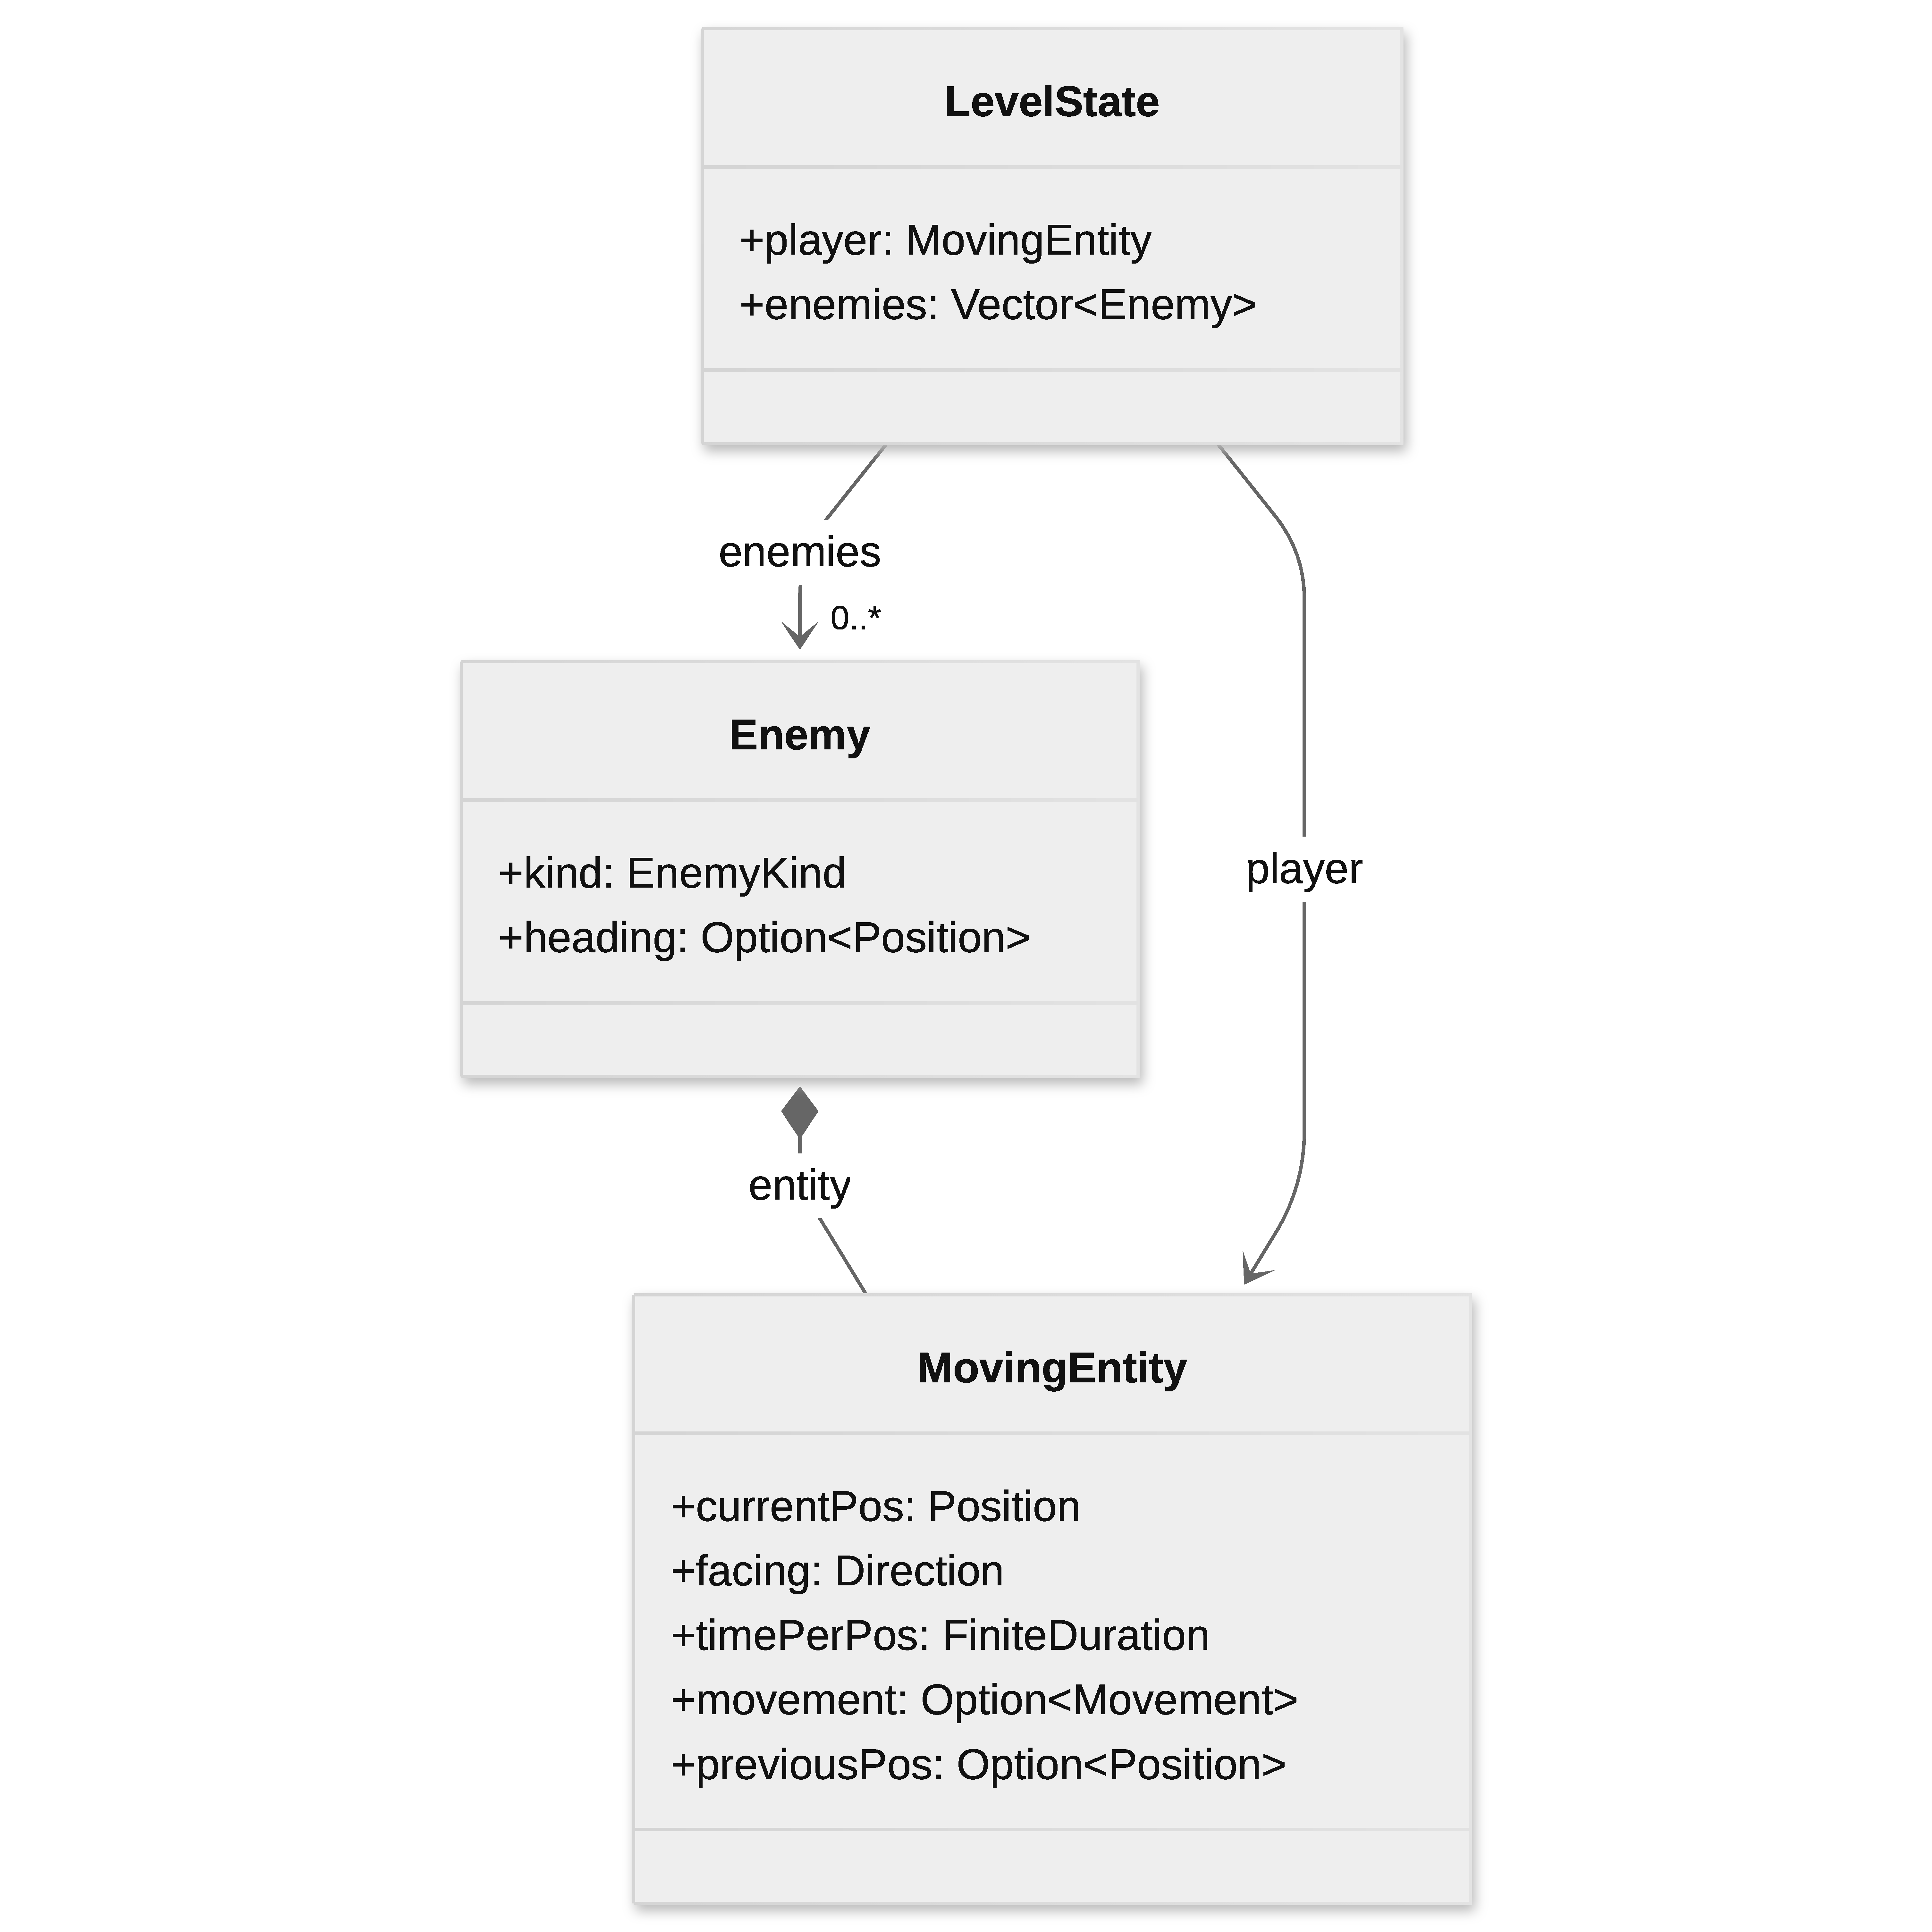
\includegraphics[width=0.8\textwidth]{../docs/uml/EntitityClassDiagram.pdf}
    \caption{An enemy is a moving entity together with its kind; the player is a moving entity and nothing more.}
\end{figure}


\subsection{Enemy behavior}

\subsection{Game modes}

\subsection{Scoring rules}

Scoring is split across three responsibilities that change for different reasons: what happened, what it is worth in
points, and how many points have been accumulated so far.

What happened is expressed as a \textbf{scoring event}: collecting a standard item, gathering a bonus item,
defeating an enemy, finishing without losing all lives, finishing with time to spare, surviving a number of waves.
Events are data that is carrying only what is needed to score them: a number of lives, a duration left, a count of
waves. The model reports that something happened without knowing what it is worth.

What it is worth is a \textbf{scoring rule}. These have been implemented through the \textbf{strategy pattern},
A rule maps an event to an amount of points, and three rules exist, one for each game mode. The pattern is used
because the modes do not simply scale the same scoring differently, but they score different events entirely. Under
the standard rule, points come from what is gathered and whom the player defeats; under the timed rule, points come
from the time remaining at the end of the game, and under the survival rule, they come from the waves outlived by
the player. An event that a rule has no interest in is worth nothing, and is not an error, so each rule stays total
over the whole event type, and they do not know which events the other handle.

The rule enforced is a property of the game mode, and reaches the scoring code as a context parameter, so no part of
the model has to carry it from hand to hand, and none of it decides which rule applies.

What has been accumulated is the \textbf{score tracker}: the points and the combo of consecutive enemy defeats.
Defeating an enemy increases the combo, and each combo increase while in the same period of invulnerability is worth
double the points of the previous one. The combo is broken once the invulnerability effect subsides. The run is kept
inside the tracker in order to allow the doubling effect, since the number of defeated enemies is not recoverable
from any single state of the game.

When a game ends, the score together with whatever the mode awards at the finish becomes a \textbf{result}: a score,
the name of the player, and the instant it was reached. That is the value the leaderboard orders and keeps.

\begin{figure}
    \centering
    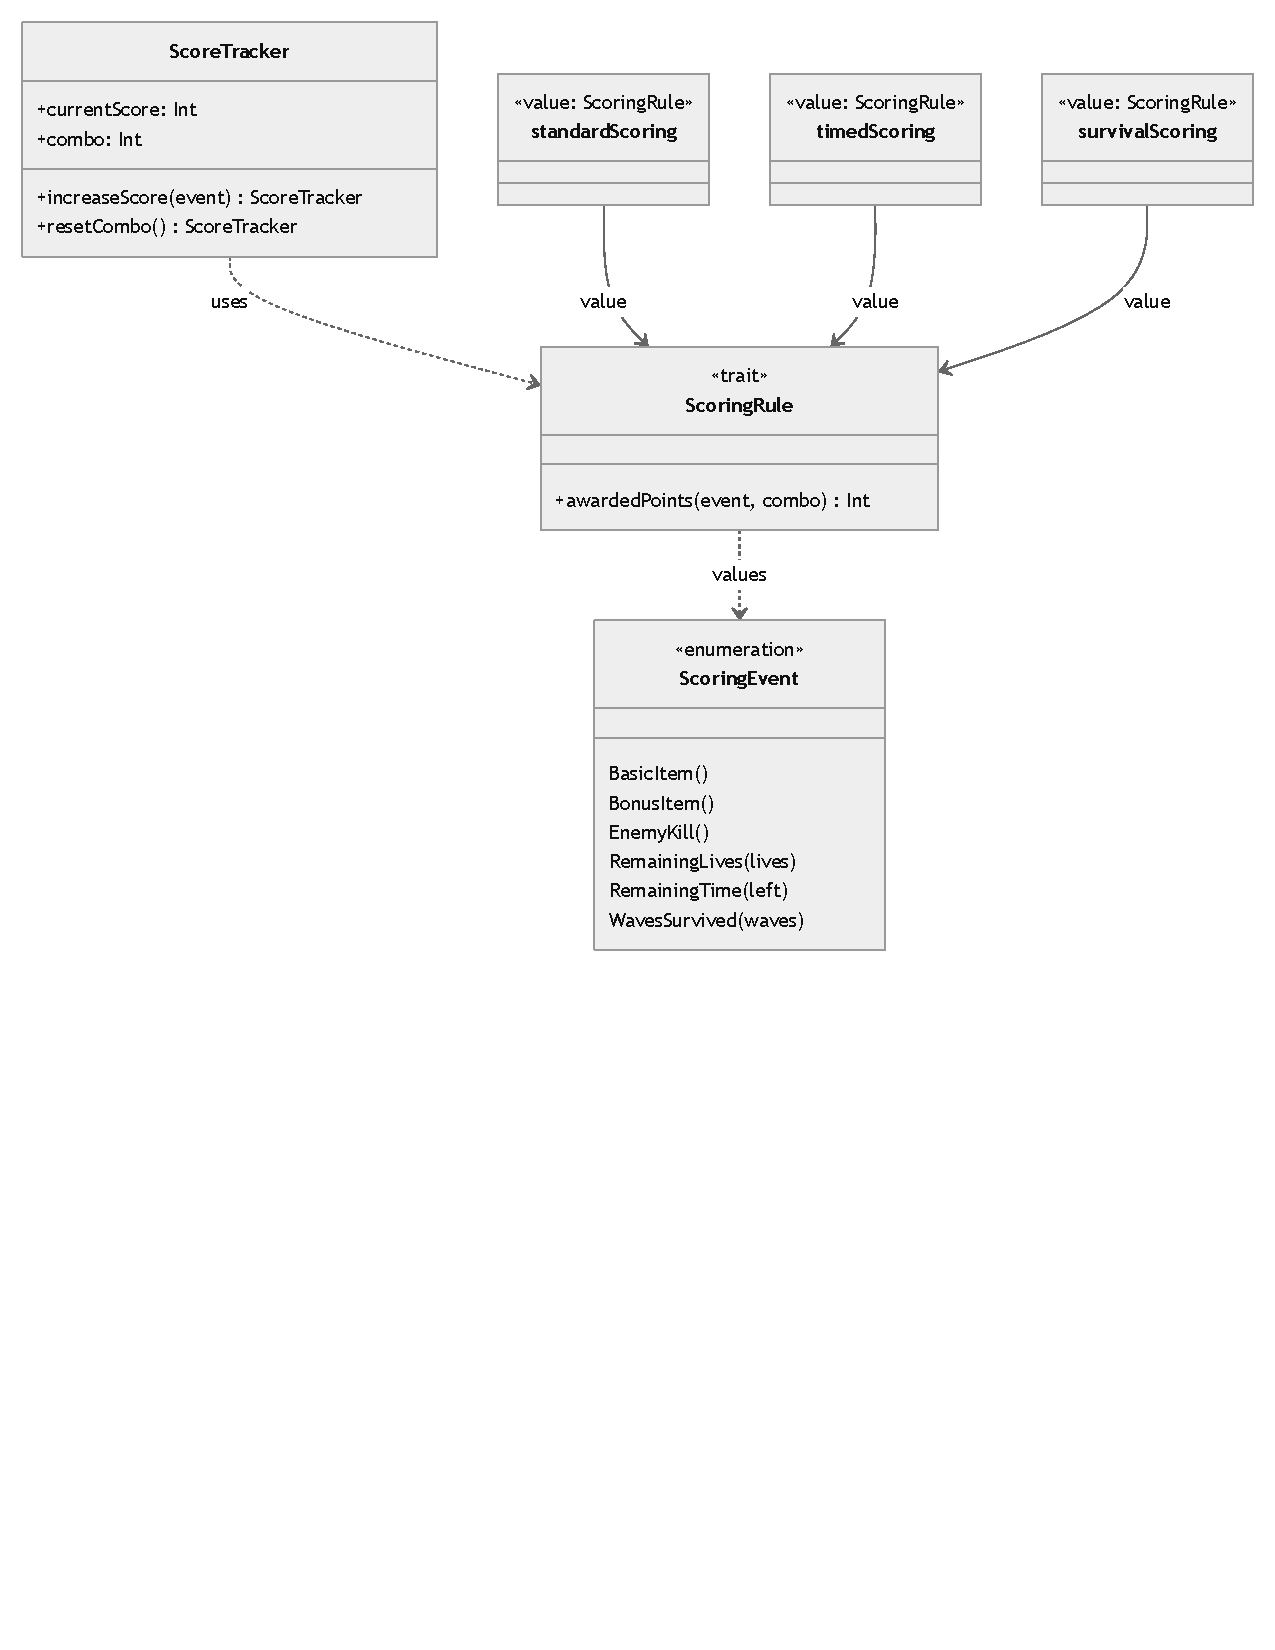
\includegraphics[width=0.8\textwidth]{../docs/uml/ScoringDiagram.pdf}
    \caption{Three interchangeable rules value the same set of events, and the tracker accumulates what they return.
    The three events carrying a value show it; the others take none.}
\end{figure}

\subsection{Leaderboard creation and updates}

A leaderboard holds the results achieved on one maze in one game mode, ordered from best to worst and no more than one
hundred deep. Results from different mazes or modes are never gathered together.

Combining two leaderboards is the only operation that changes one: recording a result means combining the leaderboard
read back from storage with a leaderboard holding the single new result. That operation was deliberately designed
to form a \textbf{monoid}, an algebraic structure consisting of a set, an associative binary operation upon it, and an
identity element for that operation. Leaderboards are the set, combining is the operation, and the empty leaderboard
is the identity. Combining is associative, so it cannot matter how results are grouped, and combining with the empty
leaderboard changes nothing.

Associativity is not free here, because combining also truncates to the best hundred. Were two results able to compare
as equal, which of them made it onto the leaderboard would depend on how the results happened to be grouped. So the
ordering is total: results rank by descending score, ties break by the moment a result was achieved, and any tie
remaining breaks by the name of whoever played.

For the construction of a leaderboard, the \textbf{smart constructor} pattern is used: the constructor is private,
and the only way to obtain a leaderboard is a factory that sorts and truncates whatever list of results it is given.
Every leaderboard is therefore already ordered and already within the cap, which is why asking for the best results
takes them from the top with no need to sort again. The invariant is established once, where the value is made, instead
of being checked wherever it is used.

A maze nobody has played has an empty leaderboard rather than no leaderboard at all. The empty value is a leaderboard
like any other, so it can be displayed, combined, asked for its best results, so no case for absence is ever carried.
This is a display of the \textbf{null object} pattern, that in this case coincides with the identity element of the monoid.

\begin{figure}
    \centering
    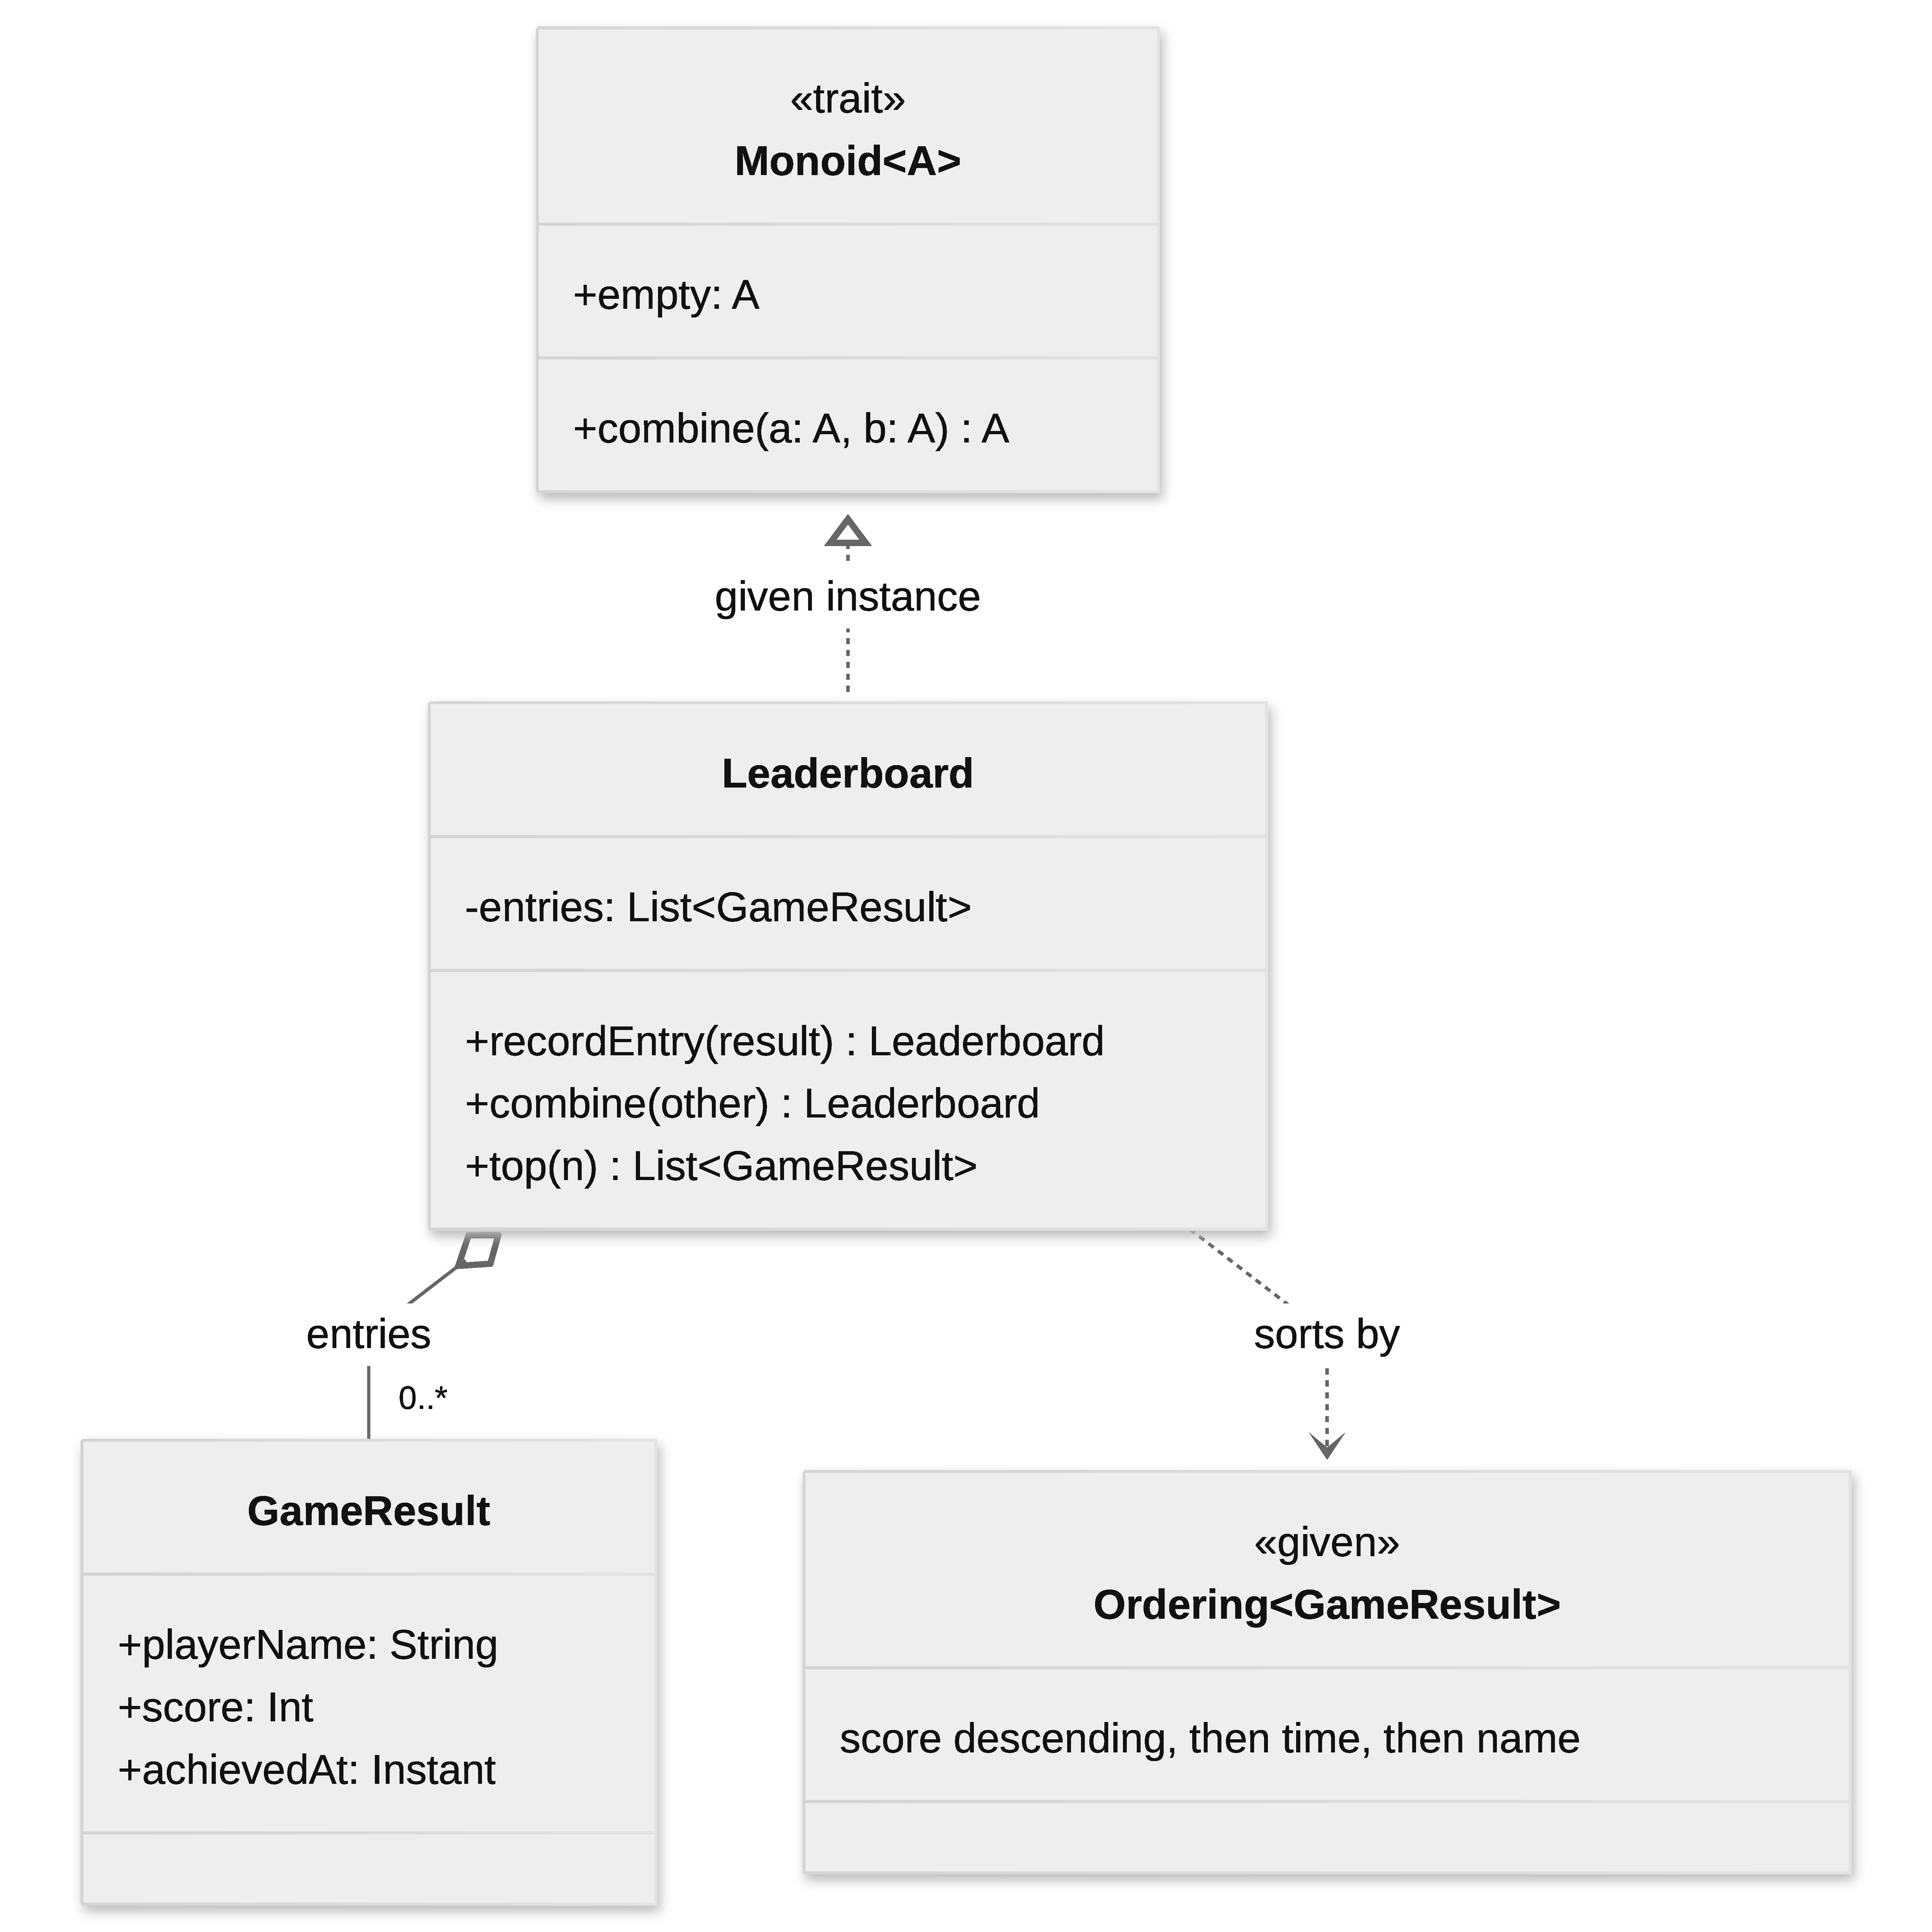
\includegraphics[width=0.8\linewidth]{../docs/uml/LeaderboardClassDiagram.pdf}
    \caption{The leaderboard as an instance of a general algebraic structure: it holds results and depends on a total ordering over them.}
\end{figure}


\subsection{Ordered updates stages}

\subsection{Game loop and game clock}

A game in progress is governed by two small values which between them decide whether time passes and how much of it has.

The \textbf{game loop} is a \textbf{finite state machine} over three states: not yet started, running, or paused. What
makes it a machine rather than a flag is that the legal transitions are declared rather than assumed. Every one of
them goes through a single guarded operation, which is told the states it may be performed from: starting is legal
only from not-yet-started, pausing only from running, resuming only from paused. Anything else is refused. The rules
therefore only live in one place and can be read off the three operations, rather than being spread over multiple
conditions where a loop is changed.

An illegal transition raises an error rather than returning a failure, because nobody playing the game can cause one:
it would mean the program itself had asked for something the machine does not allow. Starting, pausing and resuming are
therefore strict, and they are where the machine's rules are stated and where its tests reach them. The graphical
interface does not use them directly: it has an operation of its own that turns a running loop into a paused one,
and a paused loop into a running one. A pause key pressed at the wrong moment thus has no effect, and the refusals
stay reachable only from code.

\begin{figure}
    \centering
    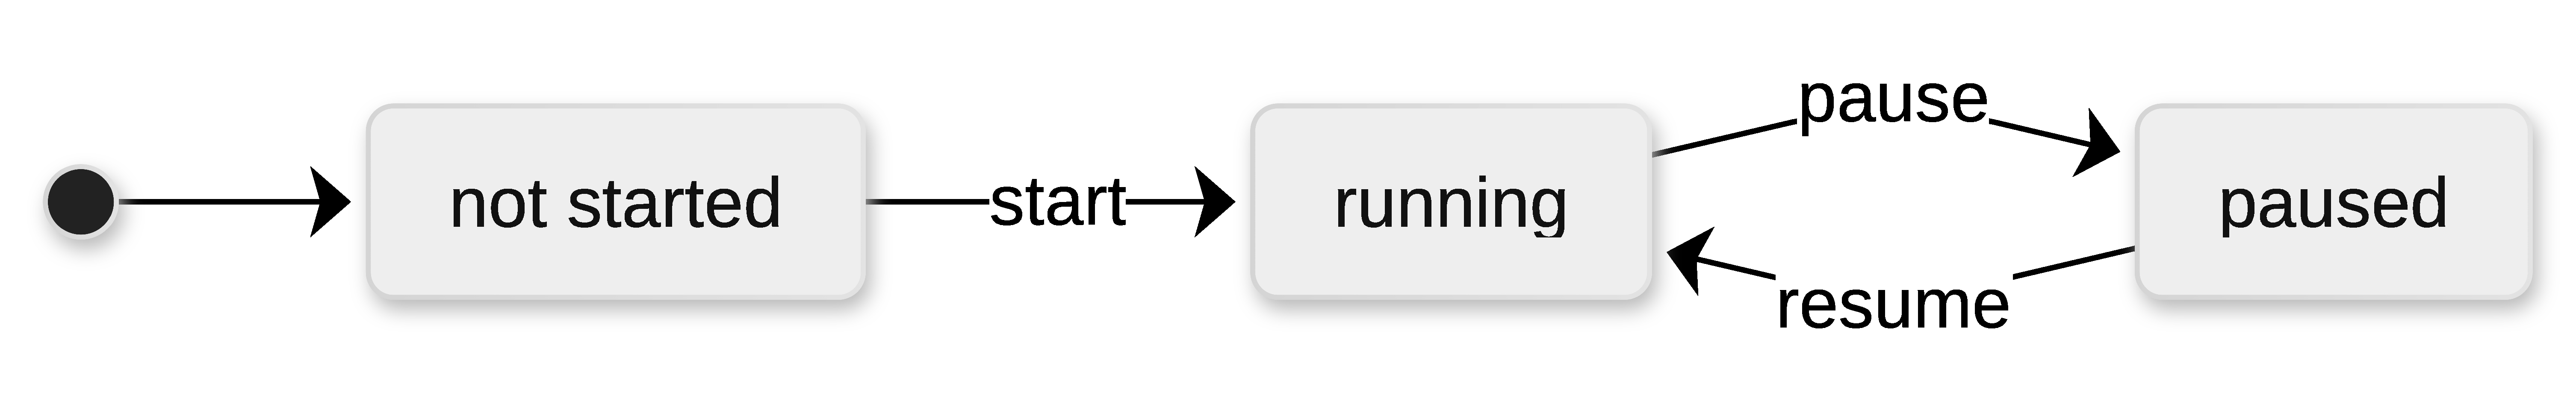
\includegraphics[width=0.6\linewidth]{../docs/uml/GameLoopStateDiagram.pdf}
    \caption{The state machine. There is no way back to \textbf{not started}, no way from it to \textbf{paused},
        and no final state: a loop is discarded rather than ended.}
\end{figure}

The \textbf{game clock} records how long a game has been played for, and nothing else. Because time is handed to
it an interval at a time rather than read from the system, how far a game has got is part of its state, so a game
saved, left and later picked up again resumes at exactly the moment it was left, and a game paused needs no rule
specifically, it is simply a game that is given no time.

\subsection{Reading a maze}

\section{View}

\subsection{Drawing from a projection}

\subsection{Screens and overlays}

\section{Controller}

\subsection{The application as a value}

\subsection{From frames to game time}

The first frame of a game yields no duration at all, since there is nothing to measure from. Every frame after it
produces the interval since the one before, and that interval is what the model is advanced by. Therefore, a session
carries the moment of the last frame it saw, which is the only thing in it that has to do with real time.

Before being passed, the interval is bounded so that it is never negative and never longer than fifty milliseconds.
The lower bound guards against a clock that appears to go backwards, while the upper bound guards against a frame
the machine took too long over, like the runtime pausing to collect memory. Without it, the frame following a long
stall would advance the game by everything that elapsed during it, expiring bonuses, jumping the difficulty in survival,
and consuming the timed game limit all between one drawing and the next. The exact number is a tuning choice, not a
derived one, high enough that the ordinary frames can pass untouched, low enough that no stall is felt.

Keys are dealt with in one place only. The arrow keys and W, A, S and D are used for the four directions, escape for
toggling through the paused and running status of the game, and any other key is discarded there rather than being
able to travel onward only to be ignored by the receiver.

A direction is not applied to the player but asked for. The level keeps the request until turning becomes possible,
so if turning is asked just before a corner is taken at the first opening rather than lost.

\subsection{Rendering with change detection}

\subsection{Adapters design}

\subsubsection{Storing a leaderboard}

Recorded results reach a file through an interface that mentions neither files nor formats: it can be asked for the
leaderboard, and it can be given one to keep. Everything about how that is done is inside a single implementation,
one file per combination of maze and mode.

A leaderboard is written as one line for each game result, containing the score, the moment it was achieved, and the
name of whoever played, separated by commas. The name is written last to allow players to have commas in their names.

Turning a result into a line and a line back into a result are two separate abilities, because not every line can be
read and converted into a game result, but every game result can be converted into a line.

When storing a game result, the leaderboard that is to receive it is first read from the storage, then combined with
the new game result, and finally saved to the storage once again, as a simple line append to the file would preserve
neither the order nor the cap of the leaderboard.

In case of a malformed leaderboard read, a failure is reported naming the first faulty line found. A missing
leaderboard file is not treated as failure: no game has yet been recorded on that maze in that mode, so the answer
is an empty leaderboard, which behaves as any other.
